\documentclass{beamer}
\usepackage{amsmath,amsbsy,amsopn,amstext,amsfonts,amssymb}
\usepackage{isomath}
\usepackage{ulem}
%\linespread{1.6}  % double spaces lines
\usepackage{graphicx}
\usepackage{subfigure}
\usepackage{color}
\usepackage{optidef}  % define optimization problems
\usepackage{multicol}  % multiple columns
\usepackage{listings} % for python code
\usepackage{mathrsfs}

\usepackage{polynom}
\newcommand{\adj}{\mathrm{adj}}
\newcommand{\constrainedmin}[3]{
		\begin{mini*}|s|
		{#2}{#1}{}{}
		\addConstraint{#3}
		\end{mini*}
}

\newcommand{\rwbcomment}[1]{{\color{blue}RWB:#1}}
\newcommand{\defeq}{\stackrel{\triangle}{=}}
\newcommand{\abs}[1]{\left|#1\right|}
\newcommand{\norm}[1]{\left\|#1\right\|}
\newcommand{\iprod}[1]{\left<#1\right>}
\newcommand{\ellbf}{\boldsymbol{\ell}}
\newcommand{\nubf}{\boldsymbol{\nu}}
\newcommand{\mubf}{\boldsymbol{\mu}}
\newcommand{\abf}{\mathbf{a}}
\newcommand{\bbf}{\mathbf{b}}
\newcommand{\cbf}{\mathbf{c}}
\newcommand{\dbf}{\mathbf{d}}
\newcommand{\ebf}{\mathbf{e}}
\newcommand{\fbf}{\mathbf{f}}
\newcommand{\gbf}{\mathbf{g}}
\newcommand{\hbf}{\mathbf{h}}
\newcommand{\ibf}{\mathbf{i}}
\newcommand{\jbf}{\mathbf{j}}
\newcommand{\kbf}{\mathbf{k}}
\newcommand{\lbf}{\mathbf{l}}
\newcommand{\mbf}{\mathbf{m}}
\newcommand{\nbf}{\mathbf{n}}
\newcommand{\obf}{\mathbf{o}}
\newcommand{\pbf}{\mathbf{p}}
\newcommand{\qbf}{\mathbf{q}}
\newcommand{\rbf}{\mathbf{r}}
\newcommand{\sbf}{\mathbf{s}}
\newcommand{\tbf}{\mathbf{t}}
\newcommand{\ubf}{\mathbf{u}}
\newcommand{\vbf}{\mathbf{v}}
\newcommand{\wbf}{\mathbf{w}}
\newcommand{\xbf}{\mathbf{x}}
\newcommand{\ybf}{\mathbf{y}}
\newcommand{\zbf}{\mathbf{z}}
\newcommand{\Jbf}{\mathbf{J}}
\newcommand{\Acal}{\mathcal{A}}
\newcommand{\Bcal}{\mathcal{B}}
\newcommand{\Lcal}{\mathcal{L}}
\newcommand{\Ncal}{\mathcal{N}}
\newcommand{\Rcal}{\mathcal{R}}
\definecolor{darkolivegreen}{rgb}{0.33, 0.42, 0.18}

\makeatletter
\newenvironment<>{proofstart}[1][\proofname]{%
    \par
    \def\insertproofname{#1\@addpunct{.}}%
    \usebeamertemplate{proof begin}#2}
  {\usebeamertemplate{proof end}}
\newenvironment<>{proofcont}{%
  \setbeamertemplate{proof begin}{\begin{block}{}}
    \par
    \usebeamertemplate{proof begin}}
  {\usebeamertemplate{proof end}}
\newenvironment<>{proofend}{%
    \par
    \pushQED{\qed}
    \setbeamertemplate{proof begin}{\begin{block}{}}
    \usebeamertemplate{proof begin}}
  {\popQED\usebeamertemplate{proof end}}
\makeatother

\title{ECEn 671: Mathematics of Signals and Systems \\ 
Moon: Chapter 6.}
\author{Randal W. Beard}
\institute{Brigham Young University}
\date{\today}

\begin{document}

%-------------------------------
\begin{frame}
	\titlepage
\end{frame}

%-------------------------------
\begin{frame}[t]
\frametitle{Table of Contents}
\tableofcontents
\end{frame}

%%%%%%%%%%%%%%%%%%%%%%%%%%%%%%%%%%%%%%%%%%%%%%%%%%%%%%%%%%%%%%%%%
\section{Eigenvalues and Eigenvectors}
\frame{\sectionpage}


%----------------------------------
\begin{frame}\frametitle{Eigenpair}
	Let $A\in\mathbb{C}^{n\times n}$.
	\begin{definition}
		\begin{itemize}
		  \item $(\lambda,x)$ is a \underline{right eigen-pair} if $Ax=\lambda x$ and $x \neq 0$.
		  \item $(\lambda,x)$ is a \underline{left eigen-pair} if $x^HA=\lambda x^H$ and $x\neq 0$.
		\end{itemize}		
	\end{definition}
	Note that $Ax = \lambda x$ can be written as
	\[ 
		(\lambda I - A)x = 0. 
	\]
	Therefore for $x$ to be an eigenvector (associated with $\lambda $) then $x\in\mathcal{N}(\lambda I-A)$, and
	\[
		x\neq 0 \Rightarrow \mathcal{N}(\lambda I-A) \neq \{0\} \Rightarrow det(\lambda I-A)=0 
	\]
	This formula can be used to find the eigenvalues and eigenvectors of a matrix.
\end{frame}

%----------------------------------
\begin{frame}\frametitle{Eigenpair: Example}
	Let $A = \begin{pmatrix}
	    0 & 1\\
	    -2 & -2
	  \end{pmatrix}$.  
	Find the eigenvalues and eigenvectors.
	
	\par\underline{Eigenvalues:}
		\[ 
		det(\lambda I - A) 
			= det\begin{pmatrix}
    				\lambda  & -1\\
   					 2 & \lambda +2
  				  \end{pmatrix} 
  			= \lambda^2 + 2\lambda  + 2 
  			= 0
  	\]
  	implies that
	\[ 
		\lambda  = -1 \pm \sqrt{1-2} 
		         = -1 \pm j 
	\]
	so that
	\[ 
		\lambda_1 = -1 + j 
		\qquad \qquad 
		\lambda_2 = -1 - j.
	\]
Which one is larger?  Note, there is no possible ordering among complex numbers.
	
\end{frame}

%----------------------------------
\begin{frame}\frametitle{Eigenpair: Example}
	\par\underline{Eigenvectors:}
	The eigenvectors can be found from the formula
	\(
		(\lambda I-A)x = 0.
	\)
	\[ 
		\lambda_1: 
			\begin{pmatrix}
	    		-1+j & -1\\
	    		2 & 1+j
	  		\end{pmatrix}
			\begin{pmatrix}
	    		x_{11}\\x_{12}
	  		\end{pmatrix}
			=
			\begin{pmatrix}
	    		0\\0
	  		\end{pmatrix}.
	\]
	Note that the rows are linearly dependent since
	\begin{align*} 
		& (-1 + j) \begin{pmatrix}
	    			-1 + j & -1
	  			  \end{pmatrix} 
	  	+ \begin{pmatrix}
	    	2 & 1+j
	  	  \end{pmatrix} \\
	  	&= 
			\begin{pmatrix}
	    		-2 & -(1+j)
	  		\end{pmatrix}
	  		+	\begin{pmatrix}
	    			2 & 1 + j
	  			\end{pmatrix} \\
	  	&= 0.
	\end{align*}
	Therefore, solving $(-1 + j)x_{11} - x_{12} = 0$ gives
	\[ 
		x_{12} = (-1+j)x_{11} 
	\]
	Let $x_{11} = 1$ then $x_{12} = -1 + j$.
	
	So 
	\[
		x_1 
			= \begin{pmatrix}
	    		1\\-1+j
	  		   \end{pmatrix}
	\]
	is an eigenvector.
\end{frame}

%----------------------------------
\begin{frame}\frametitle{Eigenpair: Example}
	\[ 
		\lambda_2: 
			\begin{pmatrix}
	    		-1-j & -1\\
	    		2 & 1-j
	  		\end{pmatrix}
			\begin{pmatrix}
	    		x_{21}\\
	    		x_{22}
	  		\end{pmatrix}
			= 
			\begin{pmatrix}
	    		0\\0
	  		\end{pmatrix}
	  \]
	Again the rows are linearly dependent so solve to get
	\(
		(-1-j)x_{21} = x_{22}
	\)
	Let $x_{21} = 1$ then $x_{22} = -1 - j$.
	
	So 
	\[
		x_2 = \begin{pmatrix}
	    		1 \\ -1 -j
	  		  \end{pmatrix}
	\]
	is an eigenvector.
\end{frame}

%----------------------------------
\begin{frame}\frametitle{Characteristic Polynomial}
	\begin{definition}
		The polynomial
		\[
			\chi_A(\lambda ) = det(\lambda I - A)
		\]
		is called the \underline{characteristic polynomial} of $A$.  The eigenvalues of $A$ are the roots of $\chi_A(\lambda )=0$.  The set of roots of $\chi_A(\lambda )=0$ is called the spectrum of $A$, denoted $\lambda (A)$.
	\end{definition}
\end{frame}

%----------------------------------
\begin{frame}\frametitle{Relationship between transfer function and state space models}

	Given a state space system:
	\begin{align*}
		\dot{x} &= Ax + Bu \\ 
		y &= Cx
	\end{align*}
	where $x\in \mathbb{R}^n$, $u \in \mathbb{R}^m$, $y \in \mathbb{R}^p$, what is the transfer function?
	
	Take the Laplace transform to get
	\begin{align*}
		sX(s) &= AX(s) + BU(s)\\
		Y(s) &= CX(s)
	\end{align*}
	
	From the first equation we get 
	\[ 
		X(s) = (sI - A)^{-1}BU(s) 
	\]
	
	From the second equation we get
	\[ 
		Y(s) = \underbrace{C(sI-A)^{-1}B}_{(p\times m) \text{ transfer matrix}}U(s) 
	\]
	
\end{frame}

%----------------------------------
\begin{frame}\frametitle{Relationship between transfer function and state space models}
	What are the poles of the system?
	\begin{align*}
		Y(s) &= C(sI-A)^{-1}BU(s) \\
		     &= \frac{C \adj(sI-A)B}{\det(sI-A)}U(s) 
	\end{align*}
	
	Therefore, the poles are when 
	\[
		det(sI-A) = 0,
	\]
	i.e. when $s$ is an eigenvalue of $A$.

	\vfill
	
	{\color{blue} 
		The poles of an LTI system and the eigenvalues of $A$ are equivalent!
	}
\end{frame}

%----------------------------------
\begin{frame}\frametitle{Generalized Eigenvalues}
	Eigenvalues and eigenvectors can be defined for more general operators than just matrices.
	
	\begin{example}
		Let $h(t)$ be the impulse response of an LTI system with Fourier transform $H(j\omega)$.
		\begin{center}
			
\includegraphics[width=0.5\textwidth]{figures/chap6_linear_system}	
		\end{center}
		Recall that if $u(t)=e^{j\omega_0 t}$ then 
		\begin{align*}
		 y(t) &= |H(j\omega_0)|e^{j\left(\omega_0 t + \angle H(j\omega_0)\right)}\\
		&= |H(j\omega_0)|e^{j\angle H(j\omega_0)}e^{j\omega_0 t}
		\end{align*}
		i.e. if a sinusoid goes in then the output will be a sinusoid of the
		same frequency but different magnitude and phase.		
	\end{example}
\end{frame}

%----------------------------------
\begin{frame}\frametitle{Generalized Eigenvalues}
	\begin{lemma}
		Let $\Acal[u] = \displaystyle \int_0^\top  h(t-\tau)u(\tau)d\tau $ then
		\[ 
			(\lambda,x) = \left( H(j\omega)e^{j\angle H(j\omega)},e^{j\omega t} \right) 
		\]
		is an eigenpair of $\Acal$.
	\end{lemma}
	\begin{proof}
		\[ 
			\Acal[e^{j\omega t}] = \left( |H(j\omega)|e^{j\angle
		    H(j\omega)}\right) e^{j\omega t}.
		\]
		
		Note that for $\Acal$ there are an uncountable infinite number of eigenpairs.		
	\end{proof}
\end{frame}

%----------------------------------
\begin{frame}\frametitle{Geometric and Algebraic Multiplicity}
	\begin{definition}
		Factor the characteristic polynomial as follows:
		\[ 
			\chi_A(\lambda) = (\lambda-\lambda_1)^{m_1}(\lambda-\lambda_2)^{m_2}\cdots(\lambda-\lambda_p)^{m_p}
		\]
		$m_i$ is the \underline{algebraic multiplicity} of eigenvalue $\lambda_i$.	
	\end{definition}
	
	\begin{definition}
		The \underline{geometric multiplicity} of eigenvalue $\lambda_i$ is defined as 
		\[
			q_i = dim(\mathcal{N}(\lambda_iI-A)).
		\]
	\end{definition}
\end{frame}

%----------------------------------
\begin{frame}\frametitle{Geometric and Algebraic Multiplicity: Example}
	Let 
	$
		A = \begin{pmatrix}
	    		1 & 0 \\
	    		0 & 1
	  		\end{pmatrix}
	$ 
	then
	\[ 
		\chi_A(\lambda) 
			= \det(\lambda I - A) 
			= \det\begin{pmatrix}
	    			\lambda-1 & 0\\
					0 & \lambda-1
	  			   \end{pmatrix} 
	  		= (\lambda-1)^2. 
	\]
	Therefore, the algebraic multiplicity of $\lambda_1 = 1$ is $m_1 = 2$.
	
	What is the geometric multiplicity?
	\[ 
		q_1 = dim(\mathcal{N}(\lambda_1I-A)) 
			= dim\left(
				\mathcal{N}
					\begin{pmatrix}
	    				0 & 0\\
						0 & 0
	  				\end{pmatrix}
	  			\right) 
	  		= dim(\mathbb{R}^2) 
	  		= 2. 
	\]
	
	Note that the eigenvectors 
	$\begin{pmatrix}
	    \alpha \\ 0
	  \end{pmatrix}$ 
	and 
	$\begin{pmatrix}
	    0\\\beta
	  \end{pmatrix}$ 
	are linearly independent!
\end{frame}

%----------------------------------
\begin{frame}\frametitle{Geometric and Algebraic Multiplicity: Example}
	Let 
	$A = \begin{pmatrix}
	    	1 & 1\\
			0 & 1
	  	  \end{pmatrix}$
 	then 
	\[ 
	\chi_A(\lambda) 
		= \det\begin{pmatrix}
	    		\lambda-1 & -1\\
				0 & \lambda-1
	  		   \end{pmatrix} 
	 	= (\lambda-1)^2
	\]
	so the algebraic multiplicity of $\lambda_1 = 1$ is $m_1 = 2$.
	
	The geometric multiplicity is
	\begin{align*}
		q_1 
			&= dim(
				\mathcal{N}\{I-A\})
			= dim(\mathcal{N}
				\begin{pmatrix}
	    			0 & -1\\
					0 & 0
	  			\end{pmatrix}) \\
	  		&= dim(\{x\in\mathbb{R}^2 \mid x_2 = 0\}) 
			= 1 \neq m_1 
	\end{align*}
	
	What are the eigenvectors assocaited with $A$?
	\[ 
		(\lambda I-A)x 
			= \begin{pmatrix}
	    		0 & 1\\
				0 & 0
	  		  \end{pmatrix}
			  \begin{pmatrix}
	    		x_{11}\\
				x_{12}
	  		  \end{pmatrix} = 
			  \begin{pmatrix}
	    		x_{12}\\
				0
	  		  \end{pmatrix}
			= \begin{pmatrix}
	    		0 \\ 0
	  		  \end{pmatrix}
			\Rightarrow x_{12} = 0 
	\]
	so $\begin{pmatrix}
	    \alpha\\0
	  \end{pmatrix}$ are the eigenvectors associated with $\lambda_1$.  There are \underline{not} two linearly independent eigenvectors.
\end{frame}

%----------------------------------
\begin{frame}\frametitle{Linearly Independent Eigenvectors}
	In general we have,
	\begin{lemma}
		Let $A \in \mathbb{C}^{n\times n}$, then there are
		$n$-linearly independent eigenvectors if and only if 
		\[
		\text{algebraic multiplicity} = \text{geometric multiplicity}
		\]
		for each eigenvalue of $A$.
	\end{lemma}
\end{frame}

%----------------------------------
\begin{frame}\frametitle{Linearly Independent Eigenvectors: Proof}
	\begin{proofstart}
		First prove that if $\lambda_i \neq \lambda_j$ then
		\[ 
			\mathcal{N}(\lambda_iI-A) \cap
			\mathcal{N}(\lambda_jI-A)
			= \{0\}. 
		\]
		
		To prove the claim, suppose not, then 
		\[ 
			\exists x \neq 0 \text{ such that } x \in \mathcal{N}(\lambda_iI-A) \text{ and } x \in \mathcal{N}(\lambda_jI-A) 
		\]
		\begin{align*}
		\iff &\qquad Ax = \lambda_i x \text{ and } Ax = \lambda_j x \\
		\iff &\qquad \lambda_ix = \lambda_jx \\
		\iff &\qquad (\lambda_i-\lambda_j)x = 0 \\
		\iff &\qquad \lambda_i = \lambda_j
		\end{align*}
		which is a contradiction.	
	\end{proofstart}
\end{frame}

%----------------------------------
\begin{frame}\frametitle{Linearly Independent Eigenvectors: Proof}

	\begin{proofend}
	
		Note that the number of linearly independent eigenvectors associated with $\lambda_i$ is the geometric multiplicity $q_i$ since we can find $q_i$ linearly independent vectors that span $\mathcal{N}(\lambda_i-A)$.
	
		\vspace{0.5cm}
			
		The previous claim shows that if $x_i \in \mathcal{N}(\lambda_iI-A)$ then $x_i \notin \mathcal{N}(\lambda_jI-A)$ which implies that there are $\sum q_i$ linearly independent eigenvectors of $A$.  Since $\sum m_i = n$, the lemma follows.
		
		\vspace{0.5cm}
		
		Note that if the eigenvalues are all distinct then $m_i = 1$.  Also since $1 \leq q_i \leq m_i$, for each $i$, we must have that the algebraic multiplicity equals the geometric multiplicity.
		
	\end{proofend}
	
\end{frame}

%----------------------------------
\begin{frame}\frametitle{Linearly Independent Eigenvectors}
	Suppose that there are $n$-linearly independent eigenvectors (where some of the eigenvalues might be repeated), then we can write
	\begin{align*}
		&
		\begin{pmatrix} 
			Ax_1 & Ax_2 & \cdots & Ax_n
		\end{pmatrix}
		= \begin{pmatrix}
 			\lambda_1x_1 & \lambda_2x_2 & \cdots & \lambda_nx_n
 		  \end{pmatrix}	 \\
 		\iff &
		A 
		\underbrace{
			\begin{pmatrix} 
				x_1 & x_2 & \cdots & x_n
		  	\end{pmatrix}
		}_S
		= \underbrace{
			\begin{pmatrix} 
				x_1 & x_2 & \cdots & x_n
		  	\end{pmatrix}
		  }_S
		  \underbrace{
		  	\begin{pmatrix}
	    		\lambda_1 & 0 & \cdots & 0 \\
	    		& \ddots \\
	    		0 & 0 & \cdots & \lambda_n
	  	  	\end{pmatrix}
	  	  }_{\Lambda} \\
	  	\iff &
	  	AS = S\Lambda
	\end{align*}
	
	Since the eigenvectors are linearly independent, $S$ is invertible.  Therefore
	\begin{align*}
		& A = S\Lambda S^{-1}  \\
		\iff & \Lambda = S^{-1}AS 
	\end{align*}
	Therefore, we say that $S$ diagonalizes $A$.
\end{frame}

%----------------------------------
\begin{frame}\frametitle{Similarity Transformation}
	\begin{definition}
		Two matrices, $A$ and $B$ are said to be \underline{similar} if
		$\exists $ an invertible $T$ such that 
		\[ 
			A = TBT^{-1}.
		\]		
	\end{definition}

	\begin{lemma}
		Similar matrices have the same \underline{eigenvalues}.	
	\end{lemma}
	\begin{proof}
		Let $(\lambda,x)$ be an eigenpair of $A$, then
		\begin{align*}
			& Ax = \lambda x\\
			\iff & TBT^{-1}x = \lambda x\\
			\iff & BT^{-1}x = \lambda T^{-1}x\\
			\iff & By = \lambda y \text{ where } y = T^{-1}x\\
			\iff & (\lambda,y) \text{ is an eigenpair of }B\\
		\end{align*}		
	\end{proof}
	\end{frame}
	
%%%%%%%%%%%%%%%%%%%%%%%%%%%%%%%%%%%%%%%%%%%%%%%%%%%%%%%%%%%%%%%%%
\section{Jordan Form}
\frame{\sectionpage}	

%----------------------------------
\begin{frame}\frametitle{Jordan Form}
	What if the algebraic multiplicity does not equal the geometric
	multiplicity? (i.e., $q_i \neq m_i$ for some eigenvalue $\lambda_i$ of $A$)?
	
	\vfill
	
	Then we cannot diagonalize $A$ using a similarity transformation.
	However we can ``almost'' diagonalize $A$.
	
	\vfill
	
	The resulting ``almost diagonal`` matrix is called the \underline{Jordan form} of $A$.	
\end{frame}

%----------------------------------
\begin{frame}\frametitle{Jordan Form, cont.}
	
	Suppose the algebraic multiplicity of $\lambda_1$ is $m_1 > 1$ but the
	geometric multiplicity is $q_1 = 1$.
	
	\vfill
	
	Then $\exists$ one linearly independent eigenvector $x_1$ s.t. $Ax_1 = \lambda_1 x_1$.
	
	\vfill
	
	Now form the following chain:
	\begin{align*}
		A\xi_{11} &= \lambda_1 \xi_{11} + x_1\\
		A\xi_{12} &= \lambda_1 \xi_{12} + \xi_{12}\\
		\vdots\\
		A \xi_{1,m_1} &= \lambda_1 \xi_{1,m_1} + \xi_{1,({m_1}-1)}
	\end{align*}
	$\xi_{11} \cdots \xi_{1,m_1}$ are called the ``generalized eigenvectors'' associated with $x_1$.	
\end{frame}

%----------------------------------
\begin{frame}\frametitle{Jordan Form, cont.}
	Note that we can write the generalized eigenvector equations as
	{\footnotesize
	\[ 
		A \begin{pmatrix}
	    	x_1 & \xi_{11} & \cdots & \xi_{1,m_1}
	  	  \end{pmatrix}
		= 
			\begin{pmatrix}
	    		x_1 & \xi_{11} & \cdots & \xi_{1,m_1}
	  		\end{pmatrix}
	  		\underbrace{
				\begin{pmatrix}
	    			\lambda_1 & 1 & \ddots \\
	    			& \lambda_1 & 1 & 0\\
	    			\ddots & & \lambda_1 & \ddots & \ddots \\
	    			& 0 & & \ddots & 1\\
	    			& & \ddots & & \lambda_1\\
	  			\end{pmatrix}
	  		}_{\text{This is called a Jordan block}}
	\]
	}

	\begin{lemma}
		If the geometric multiplicity of $\lambda_i$ is $q_i = 1$ then the associated $m_1-1$ generalized 	eigenvectors are linearly independent of the other eigenvectors.
	\end{lemma}
\end{frame}

%----------------------------------
\begin{frame}\frametitle{Jordan Form, cont.}
	If $1 < q_i < m_i$ then the problem is slightly more complicated. 
	
	\vfill
	
	There are precisely $q_i$ linearly independent eigenvectors associated
	with $\lambda_i$ and there will be $q_i$ Jordan blocks associated with
	$\lambda_i$.  What are the sizes of the Jordan blocks?  For example,
	suppose $m_i = 4$ and $q_i = 2$, the possible Jordan blocks are:
	{\footnotesize
		\[ 
			\begin{pmatrix}
		    	\lambda_1 & 1 & 0\\
		    	0 & \lambda_1 & 1\\
		    	0 & 0 & \lambda_1
		  	\end{pmatrix} 
		  	\text{ and }
			\begin{pmatrix}
		    	\lambda_1
		  	\end{pmatrix}
		  	\text{ i.e., } 
			\begin{pmatrix}
		    	\lambda_1 & 1 & 0 & 0\\
		    	0 & \lambda_1 & 1 & 0\\
		    	0 & 0 & \lambda_1 & 0\\
		    	0 & 0 & 0 & \lambda_1
		  	\end{pmatrix}
		  	\text{ or }
		  	\begin{pmatrix}
		    	\lambda_1 & 0 & 0 & 0\\
		    	0 & \lambda_1 & 1 & 0\\
		    	0 & 0 & \lambda_1 & 1\\
		    	0 & 0 & 0 & \lambda_1
		  	\end{pmatrix}
		\]
	}
	or
	\[ 
		\begin{pmatrix}
	    	\lambda_1 & 1\\
	    	0 & \lambda_1
	  	\end{pmatrix} 
	  	\text{ and }
		\begin{pmatrix}
	    	\lambda_1 & 1\\
	    	0 & \lambda_1
	  	\end{pmatrix}
	  	\text{ i.e., }
	  	\begin{pmatrix}
	    	\lambda_1 & 1 & 0 & 0\\
	    	0 & \lambda_1 & 0 & 0\\
	    	0 & 0 & \lambda_1 & 1\\
	    	0 & 0 & 0 & \lambda_1	  		
	  	\end{pmatrix}
	\]	
	Which option is correct?	
\end{frame}

%----------------------------------
\begin{frame}\frametitle{Jordan Form, cont.}
	To decide, generate the generalized eigenvector for each eigenvector
	and pick the linearly independent ones.
	
	Example:  Let
	\[ 
		A = \begin{pmatrix}
	    		1 & 1 & -1 & 1\\
	    		0 & 1 & 0 & 1\\
	    		0 & 0 & 1 & 1\\
	    		0 & 0 & 0 & 1
	  		\end{pmatrix}
	\]
	Since $\det(\lambda I - A) = (\lambda-1)^4$ we have $\lambda_1 = 1$
	and $m_1 = 4$.
	\[ 
		q_1 = dim(\mathcal{N}
				\begin{pmatrix}
	    			0 & -1 & 1 & -1\\
	    			0 & 0 & 0 & -1\\
	    			0 & 0 & 0 & -1\\
	    			0 & 0 & 0 & 0
	  			\end{pmatrix}
	  		   ) 
	  		= 2
	\] 
	since there are 2 linearly independent rows.
	
\end{frame}

%----------------------------------
\begin{frame}\frametitle{Jordan Form, cont.}
	So there are two linearly independent eigenvectors:
	\[ 
		(\lambda_1I-A)x_1 
			= \begin{pmatrix}
	    		0 & -1 & 1 & -1\\
	    		0 & 0 & 0 & -1\\
	    		0 & 0 & 0 & -1\\
	    		0 & 0 & 0 & 0
	  		  \end{pmatrix}
	  		  \begin{pmatrix}
	    			x_{11}\\x_{12}\\x_{13}\\x_{14}
	  		  \end{pmatrix}
	  		= \begin{pmatrix}
	    		-x_{12} + x_{13} - x_{14}\\-x_{14}\\-x_{14}\\0
	  		  \end{pmatrix}
	  		= \begin{pmatrix}
	    		0\\0\\0\\0
	  		  \end{pmatrix}
	\]
	\[ 
		\implies x_{14} = 0 \text{ and } -x_{12}+x_{13}-x_{14} = 0 
	\]
	so
	\[ 	
		x_1 = \begin{pmatrix}
	    		1\\0\\0\\0
	  		  \end{pmatrix} 
	  	\text{ is an eigenvector, and so is } 
	  	x_2 = \begin{pmatrix}
	    		0\\1\\1\\0
	  		  \end{pmatrix}
	\]	
\end{frame}

%----------------------------------
\begin{frame}\frametitle{Jordan Form, cont.}
	Find the possible generalized eigenvector associated with eigenvector $x_1$:
	\[
		A\xi_{11} = \xi_{11}+x_1 \Rightarrow (\lambda_1 I - A)\xi_{11} = -x_1 
	\]
	\[ 
		\text{i.e. } -\xi_{112} + \xi_{113} - \xi_{114} = 1 \qquad \qquad \xi_{114} = 0 
	\]
	\[ 
		\xi_{112} = \xi_{113} + 1 
		\qquad \text{ so } \qquad 
		\xi_{11} = \begin{pmatrix}1 \\ 2\\ 1 \\ 0 \end{pmatrix} 
		\text{ is valid } 
	\]
	\[ 
		(\lambda_1I-A)\xi_{12} = \xi_{12} 
		\text{ so } 
		\begin{pmatrix}
	    	-\xi_{122} + \xi_{123} - \xi_{124} \\ -\xi_{124} \\ -\xi_{124}
	  	\end{pmatrix}
	  	= \begin{pmatrix}
	    	1\\2\\1\\0
	  	  \end{pmatrix} 
	  	\leftarrow \text{ can't use }. 
	\]	
\end{frame}

%----------------------------------
\begin{frame}\frametitle{Jordan Form, cont.}
	
	{\bf Note:}
		There are an infinite number of possibilities of generalized eigenvectors from each true eigenvector, but you can only pick ones that are linearly independent.  This second eigenvector forms a linearly dependent subset of one of the real eigenvectors.

	\vfill
	
	Therefore, one Jordan block is of size 2.
	
	\vfill
	
	Also solve $(\lambda_1I-A)\xi_{21} = x_2$ i.e.
	\[ 
		\begin{pmatrix}
	    	-\xi_{212} + \xi_{213} - \xi_{214} \\ -\xi_{214} \\ -\xi_{214} \\ 0
	  	\end{pmatrix}
	  	= \begin{pmatrix}
	    	0\\1\\1\\0
	  	  \end{pmatrix}
	  	\Rightarrow \xi_{214} = 1, \xi_{213} = \xi_{212} + 1 
	\]
	so 
	\(
		\xi_{21} = \begin{pmatrix} 0\\1\\2\\1 \end{pmatrix}.
	\)
\end{frame}

%----------------------------------
\begin{frame}\frametitle{Jordan Form, cont.}
	In summary
	\[ 
		A
		\underbrace{
			\begin{pmatrix}
	    		x_1 & \xi_{11} & x_2 & \xi_{21}
	    	\end{pmatrix}
	    }_{S} 
	    = 
	    \underbrace{
	    	\begin{pmatrix}
	    		x_1 & \xi_{11} & x_2 & \xi_{21}
	  		\end{pmatrix}
	  	}_{S}
	  	\underbrace{
	  		\begin{pmatrix}
	  			1& 1 & 0 & 0\\
	  			0 & 1 & 0 & 0\\
	  			0 & 0 & 1 & 1\\
	  			0 & 0 & 0 & 1
			\end{pmatrix}
		}_{J} 
	\]
	or
	\[ 
		A = SJS^{-1} 
	\]
	$J$ is called the ``Jordan'' form of $A$
	
	\vfill
	
	If the eigenvalues are distinct or $q_i = m_i$ for each $i$ then $J =
	\Lambda$ (is diagonal).
	
	\vfill
	
	Otherwise $J$ is block diagonal with Jordan blocks along the diagonal
	($q_i$ Jordan blocks for each eigenvalue).	
\end{frame}

%----------------------------------
\begin{frame}\frametitle{Jordan Form, cont.}
	
	Example:  suppose there are 3 eigenvalues with $\lambda_1 = 1,
	\lambda_2 = 2, \lambda_3 = 3$, and $m_1=1, m_2=2, m_3=3$, and $q_1 =
	1, q_2 = 1, q_3 = 2$.
	There are two possible Jordan forms:
	\[
	\begin{pmatrix}
	    \lambda_1\\
	    & \lambda_2 & 1 && 0\\
	    & & \lambda_2 & &\\
	    &  & & \lambda_3 & 1\\
	    & 0& & & \lambda_3\\
	    & & & & & \lambda_3
	  \end{pmatrix} \text{ or } 
	\begin{pmatrix}
	    \lambda_1\\
	    & \lambda_2 & 1 && 0\\
	    & & \lambda_2 & & \\
	    & & & \lambda_3\\
	    &0 & & & \lambda_3 & 1\\
	    & & & & & \lambda_3
	  \end{pmatrix}
	\]
\end{frame}

%%%%%%%%%%%%%%%%%%%%%%%%%%%%%%%%%%%%%%%%%%%%%%%%%%%%%%%%%%%%%%%%%
\section{Cayley-Hamilton Theorem}
\frame{\sectionpage}


%----------------------------------
\begin{frame}\frametitle{Functions of Matrices}
	\begin{lemma}
	A square matrix can always be put in Jordan form.	
	\end{lemma}
	This implies that we can always write
	\[ 
		A = SJS^{-1} 
	\]
	
	This implies that 
	\begin{align*}
		A^k &= \underbrace{AA\cdots A}_{k\text{ times}} \\
		    &= SJS^{-1}SJS^{-1}\cdots SJS^{-1} \\
		    &= SJ^kS^{-1} 
	\end{align*}
	This is particularly simple if $J = \Lambda$ since 
	\[ 
		A^k = S\Lambda^kS^{-1} 
		\text{ where } 
		\Lambda^k 
			= \begin{pmatrix}
	    		\lambda_1^k & & 0\\
	    		& \ddots \\
	    		0 & & \lambda_n^k
	  		  \end{pmatrix} 
	\]	
\end{frame}

%----------------------------------
\begin{frame}\frametitle{Functions of Matrices, cont.}
	For square matrices we can define analytic functions of matrices.
	Analytic functions are functions that can be expanded as a Taylor
	seires, e.g.
	\begin{align*}
		e^x &= 1 + x + \frac{x^2}{2!} + \frac{x^3}{3!} + \cdots \\
		\cos(x) &= 1 - \frac{x^2}{2!} + \frac{x^4}{4!} + \frac{x^6}{6!} + \cdots \\
		\sin(x) &= x - \frac{x^3}{3!} + \frac{x^5}{5!} - \frac{x^7}{7!} + \cdots 
	\end{align*}
	The corresponding Matrix function is defined in terms of its Taylor
	series, e.g.,
	\begin{align*}
		e^A &= I + A + \frac{A^2}{2!} + \frac{A^3}{3!} + \cdots\\
		\cos(A) &= I - \frac{A^2}{2!} + \frac{A^4}{4!} - \frac{A^6}{6!} + \cdots\\
		\sin(A) &= A - \frac{A^3}{3!} + \frac{A^5}{5!} - \frac{A^7}{7!} + \cdots
	\end{align*}

\end{frame}

%----------------------------------
\begin{frame}\frametitle{Cayley-Hamilton Theorem}
	Computing infinite series of matrices is a pain.  Fortunately we have
	the following theorem:
	
	\begin{theorem}[Cayley-Hamilton Theorem]
		Every matrix satisfies its own characteristic polynomial, i.e.
		\[ 
			\chi_A(A) = 0.
		\]	
	\end{theorem}
\end{frame}

%----------------------------------
\begin{frame}\frametitle{Cayley-Hamilton Theorem, proof}
	The proof holds for all $A$ but we will only prove the case when
	$q_i=m_i$ for each $\lambda_i$.  In this case $A=S\Lambda S^{-1}$.
	Note that for each eigenvalue $\chi_A(\lambda_i) = 0 $ since
	$\chi_A(\lambda_i) = \det(\lambda_i I - A)$
	
	Let \[
			\chi_A(\lambda) = \lambda^n + a_{n-1}\lambda^{n-1} + \cdots + a_1\lambda + a_0 
		\]
	then
	\begin{align*}
		\chi_A(A) &= A^n + a_{n-1}A^{n-1} + \cdots + a_1A + a_0I \\
				  &= S\Lambda^nS^{-1} + a_{n-1}S\Lambda^{n-1}S^{-1} + \cdots + a_1S\Lambda S^{-1} + a_0SS^{-1}\\
				  &= S(\Lambda^n + a_{n-1}\Lambda^{n-1} + \cdots + a_1\Lambda + a_0I)S^{-1}
	\end{align*}
	Note that the matrix 
	\[
		\Lambda^n + a_{n-1}\Lambda^{n-1} + \cdots + a_1\Lambda + a_0I
	\]
	is diagonal with each element on the diagonal equal to $\lambda_i^n +
	    a_{n-1}\lambda_i^{n-1} + \cdots + a_1\lambda_i + a_0=0$.
	  
	Therefore 
	\[
		\Lambda^n + a_{n-1}\Lambda^{n-1} + \cdots + a_1\Lambda + a_0I = 0.
	\]	
\end{frame}

%----------------------------------
\begin{frame}\frametitle{Cayley-Hamilton Theorem, implications}
	{\footnotesize
		Recall polynomial division:
		\begin{align*}
			& \frac{f(x)}{q(x)} = a(x) + \frac{r(x)}{q(x)} \\
			\implies & 
				\underbrace{f(x)}_{\text{degree $m$}} 
					=
					\underbrace{a(x)}_{\text{degree $(m-n)$}}
					\overbrace{q(x)}^{\text{degree $n$}} 
					+ \underbrace{r(x)}_{\text{degree $< n$}}
		\end{align*}
		Application to infinite series like $e^x$ gives
		\[ 
			\underbrace{e^x}_{\text{degree $\infty$}} 
				= \underbrace{a(x)}_{\text{degree $\infty$}}
				  \overbrace{\chi_A(x)}^{\text{degree $n$}} 
				  + \underbrace{r(x)}_{\text{degree $<n$}}
		\]
	}
	Since $\chi_A(A) = 0$,
	\begin{align*}
	 	e^A &= \underbrace{r(A)}_{\text{degree $< n$}}
			&= \cdots b_{n-1}A^{n-1} + \cdots + b_1A + b_0I
	\end{align*}
	Since $e^{\lambda_i} = r(\lambda_i)$ the coefficients can be found
	from
	\[ 
		e^{\lambda_i} = \cdots b_{n-1}\lambda^{n-1} + \cdots + b_1\lambda + b_0.
	\]	
\end{frame}

%----------------------------------
\begin{frame}\frametitle{Cayley-Hamilton Theorem, example}
	Find $e^A$ where 
	$A = \begin{pmatrix}
	    	0 & 1\\
	    	-2 & -2
	  	  \end{pmatrix}$.  
	{\footnotesize
	\[ \det(\lambda I - A ) = \lambda^2 + 2\lambda + 2 \Rightarrow
	\lambda_{1,2} = -1 \pm j \]
	\[ \Rightarrow e^A = b_1A + b_0I = \begin{pmatrix}
	    0 & b_1\\
	    -2b_1 & -2b_1
	  \end{pmatrix}+\begin{pmatrix}
	    b_0 & 0\\
	    0 & b_0
	  \end{pmatrix} = \begin{pmatrix}
	    b_0 & b_1\\
	    -2b_1 & -2b_1-b_0
	  \end{pmatrix}\]
	}
	where $b_0$ and $b_1$ satisfy
	\[e^{-1+j} = b_1(-1+j) + b_0\]
	\[e^{-1-j} = b_1(-1-j)+b_0 \]
	\[ \Rightarrow \begin{pmatrix}
	    b_0\\b_1
	  \end{pmatrix}
	= \begin{pmatrix}
	    1 & -1+j\\
	    1 & -1-j
	  \end{pmatrix}^{-1}\begin{pmatrix}
	    e^{-1+j}\\e^{-1-j}
	  \end{pmatrix}=\begin{pmatrix}
	    0.5083\\
	    0.3096
	  \end{pmatrix}
	\]
	\[\Rightarrow e^{A} = \begin{pmatrix}
	    0.5083 & 0.3096\\
	    -0.6191 & -0.1108
	  \end{pmatrix}
	 \]
\end{frame}


%%%%%%%%%%%%%%%%%%%%%%%%%%%%%%%%%%%%%%%%%%%%%%%%%%%%%%%%%%%%%%%%%
\section{Self Adjoint Matrices}
\frame{\sectionpage}

%----------------------------------
\begin{frame}\frametitle{Self Adjoint Matrices}
	\begin{definition}
	A matrix $A\in\mathbb{C}^{n\times n}$ is said to be \underline{self adjoint} (also called \underline{Hermitian}) if 
	\[
		A = A^H.
	\]	
	\end{definition}
	
	\begin{lemma}[Moon 6.2]
 		If $A = A^H$ then the eigenvalues of $A$ are real.
	\end{lemma}
	\begin{proof}
		Let $(\lambda,x)$ be a right eigen-pair, then
		\[ 
			Ax = \lambda x, \text{ and } x^HA^H = \bar{\lambda}x^H.
		\]
		Therefore 
		\begin{align*}
			& x^HAx = \lambda x^Hx, \text{ and } x^HA^Hx = \bar{\lambda}x^Hx \\
			\implies & \lambda x^Hx = \bar{\lambda}x^Hx  
			\implies  \bar{\lambda} = \lambda, \\
			\implies & \lambda \text{ is real. }	
		\end{align*}
	\end{proof}
\end{frame}

%----------------------------------
\begin{frame}\frametitle{Self Adjoint Matrices}
	\begin{lemma}[Moon 6.3]
		If $A=A^H$ and the eigenvalues are distinct, then the eigenvectors are orthogonal.
	\end{lemma}
	
	\begin{proof}
	Let $(\lambda_1,x_1)$ and $(\lambda_2,x_2)$ be distinct eigenpairs, i.e. $\lambda_1 \neq \lambda_2$, then
	\begin{align*}
		& x_2^HAx_1 = \lambda_1x_2^Hx_1 \\
		\text{and~} & x_2^HA^Hx_1 = \lambda_2x_2^Hx_1 \
	\end{align*}
	Therefore $(\lambda_1-\lambda_2)x_2^Hx_1 = 0$.
	Because $\lambda_1 \neq \lambda_2$ we must have that
	\[
		x_2^Hx_1 = 0
	\]
	which implies that $x_1$ and $x_2$ are orthogonal.
	\end{proof}
	{\color{blue}
		Note the eigenvectors can always be chosen to be orthonormal.
	}
\end{frame}

%----------------------------------
\begin{frame}\frametitle{Self Adjoint Matrices}

	\begin{theorem}[Moon Theorem 6.2 (Special Theorem)]
		If $A\in\mathbb{C}^{n\times n}$ is Hermitian,
		then $q_i = m_i$ for each eigenvalue $\lambda_i$.
	\end{theorem}
	
	\begin{corollary}
		If $A=A^H$, then $\exists$ a unitary $U$ and real diagonal $\Lambda$ such that
		\[
			A = U \Lambda U^H.
		\]
	\end{corollary}
	
\end{frame}

%----------------------------------
\begin{frame}\frametitle{Eigenvalues and Rank}
	
	\begin{lemma}[Moon Lemma 6.5]
		Let $A \in \mathbb{C}^{m\times m}$ be of rank $r < m$.  Then at least $m- r$ of the eigenvalues of $A$ are equal to zero	
	\end{lemma}
\end{frame}





%%%%%%%%%%%%%%%%%%%%%%%%%%%%%%%%%%%%%%%%%%%%%%%%%%%%%%%%%%%%%%%%%
\section{Invariant Subspaces}
\frame{\sectionpage}

%----------------------------------
\begin{frame}\frametitle{Invariant Subspaces}
	\begin{definition}
		Let $A$ be a square matrix.  
		If $\mathbb{S} \subset \mathcal{R}(A)$ is such that $x \in \mathbb{S} \implies Ax \in \mathbb{S}$ then $\mathbb{S}$ is an \underline{invariant subspace} of $A$.
	\end{definition}
	
	\begin{example}
		An eigenvector forms an invariant subspace i.e. 
		\[
			\mathbb{S} = \{\alpha x \mid x \text{~is an eigenvector}\}
		\]
		is invariant since $\hat{x} \in \mathbb{S} \Rightarrow A\hat{x} = \lambda\hat{x} \in \mathbb{S}$.		
		\end{example}
\end{frame}

%----------------------------------
\begin{frame}\frametitle{Invariant Subspaces}
	\begin{example}
		The span of any subset of eigenvectors is invariant:  Let $x_1 \ldots x_p$ be eigenvectors with associated eigenvalues $\lambda_1 \ldots \lambda_p$.
		
		Let 
		\[
			\mathbb{S} = \text{span}\{x_1 \ldots x_p\}
		\]
		then
		\begin{align*}
			& \hat{x} \in \mathbb{S} \\
			\implies & \hat{x} = \alpha_1 x_1 + \cdots + \alpha_p x_p \\
			\implies & A\hat{x} = \alpha_1Ax_1 + \cdots + \alpha_pAx_p \\
			\implies & A\hat{x} = \alpha_1\lambda_1x_1 + \cdots + \lambda_p\alpha_px_p \\
			\implies & A\hat{x} \in \mathbb{S}.		
		\end{align*}
	\end{example}
\end{frame}

%----------------------------------
\begin{frame}\frametitle{Applications to Differential Equations}
	Consider the differential equation 
	\(
		\dot{x} = Ax
	\)
	with initial condition $x(0)=x_0$.
	\begin{lemma}
	 	The solution is given by
	 	\(
	 		x(t) = e^{At}x_0
	 	\)
	 	where $e^{At} = I + At + \frac{1}{2!}A^2t^2 + \frac{1}{3!}A^3t^3 + \cdots$.
	\end{lemma}
	\begin{proof}
		{\footnotesize
		Plug into equation
		\begin{align*}
			\frac{dx(t)}{dt} 
				&= \frac{d}{dt}(e^{At})x_0 + e^{At}\frac{d}{dt}(x_0) 
				= \frac{d}{dt}e^{At}x_0\\
				&= \frac{d}{dt}(I + At + \frac{A^2t^2}{2!} + \frac{A^3t^3}{3!} + \frac{A^4t^4}{4!} + \cdots x_0\\
				&= (A + A^2t + \frac{A^3t^2}{2!} + \frac{A^4t^3}{3!} + \cdots)x_0\\
				&= A(I + At + \frac{A^2t^2}{2!} + \frac{A^3t^3}{3!} + \cdots)x_0\\
				&= Ae^{At}x_0
				= Ax(t)
		\end{align*}
		so $x(t) = e^{At}x_0$ satisfies $\dot{x} = Ax$ with initial condition $x_0$.
		}
	\end{proof}
\end{frame}

%----------------------------------
\begin{frame}\frametitle{Applications to Differential Equations}
	\begin{lemma}
		If $\mathbb{S}$ is an invariant subspace of $A$ then $\mathbb{S}$ is an invariant subspace of $e^{At}$
	\end{lemma}
	\begin{proof}
		Let $x_0 \in \mathbb{S}$ then
		\begin{align*}
			Ax_0 \in \mathbb{S} 
				&\implies tAx_0 \in \mathbb{S} \\
				&\implies A(Ax_0) \in \mathbb{S} \\
				&\implies \frac{A^2t^2}{2!}x_0 \in \mathbb{S} \\
				&\ldots
		\end{align*}
		Therefore
		\[
			x(t) = Ix_0 + Atx_0 + \frac{A^2t^2}{2!}x_0 + \frac{A^3t^3}{3!}x_0 + \cdots \in \mathbb{S}.
		\]
	\end{proof}
\end{frame}

%----------------------------------
\begin{frame}\frametitle{Applications to Differential Equations: Example}
	Consider the differential equation
	\[
		\dot{x} 
			= \begin{pmatrix}
	    		0 & 1\\
	    		2 & -1
	  		  \end{pmatrix} x.
	\]
	The eigenvalues of $A$ are given by
	\(
		\text{det}(\lambda I - \begin{pmatrix}
	    							0 & 1\\
	    							2 & -1
	  							\end{pmatrix}) 
	  	= (\lambda - 1)(\lambda + 2) = 0
	\)
	and so $\lambda_1 = 1$ and $\lambda_2 = -2$.
	
	\vfill
	
	The associated eigenvector are
	\[ 
		x_1 = \begin{pmatrix} 1 \\ 1 \end{pmatrix} 
		\text{ and }
		x_2 =  \begin{pmatrix} 1 \\ -2 \end{pmatrix}.
	\]
\end{frame}

%----------------------------------
\begin{frame}\frametitle{Applications to Differential Equations: Example}
	\begin{center}
		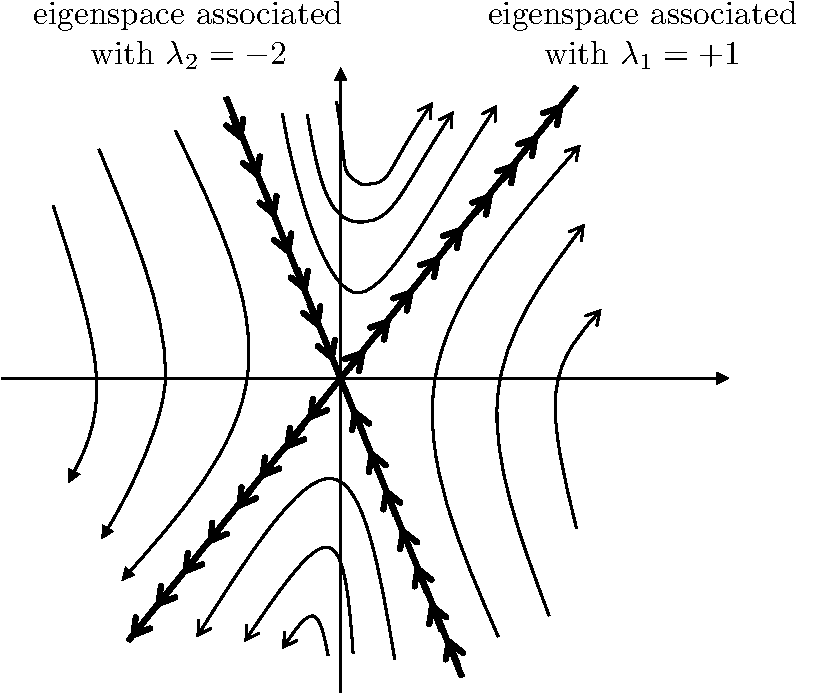
\includegraphics[width=0.7\textwidth]{figures/chap6_invariant_subspaces}
	\end{center}
	
	\begin{itemize}
		\item 	If the initial condition is on $span\{x_1\}$, then the solution remains on $span\{x_1\}$.
		\item If the initial condition is on $span\{x_2\}$, then the solution remains on $span\{x_2\}$.
		\item Otherwise it is a combination of the two modes.
	\end{itemize}
\end{frame}

%----------------------------------
\begin{frame}\frametitle{Applications to Difference Equations: Example}

	\rwbcomment{Change system to eigenvalues in unit circle.  Show that eigenspaces are invariant.  Provide example.}

	Consider the differential equation
	\[
		x[k+1] 
			= \begin{pmatrix}
	    		0 & 1\\
	    		2 & -1
	  		  \end{pmatrix} x[k].
	\]
	Again the eigenvalues of $A$ are $\lambda_1 = 1$ and $\lambda_2 = -2$, and the eigenvectors are
	\[ 
		x_1 = \begin{pmatrix} 1 \\ 1 \end{pmatrix} 
		\quad \text{ and } \quad
		x_2 =  \begin{pmatrix} 1 \\ -2 \end{pmatrix}.
	\]
		
\end{frame}


%%%%%%%%%%%%%%%%%%%%%%%%%%%%%%%%%%%%%%%%%%%%%%%%%%%%%%%%%%%%%%%%%
\section{Quadratic Forms}
\frame{\sectionpage}

%----------------------------------
\begin{frame}\frametitle{Quadratic Forms}
	\begin{definition}
		A real square matrix is \underline{symmetric} if $A^\top =A$	
	\end{definition}
	
	\begin{definition}
		A real square matrix is \underline{skew-symmetric} if $A^\top  = -A$
	\end{definition}
\end{frame}

%----------------------------------
\begin{frame}\frametitle{Quadratic Forms}
	\begin{lemma}
		Any real square matrix $B\in\mathbb{R}^{n\times n}$ can be written as
		\[ 
			B = B_s + B_{ss} 
		\]
		where $B_s$ is symmetric and $B_{ss}$ is skew-symmetric.
	\end{lemma}
	
	\begin{proof}
		\begin{align*}
			B &= \frac{B + B^\top }{2} + \frac{B - B^\top }{2} 
			  \defeq  B_s + B_{ss} 
		\end{align*}
		where
		\begin{align*}
			B_s^\top  &= \left(\frac{B + B^\top }{2}\right)^\top  
			      = \frac{B^\top  - B}{2} = \frac{B + B^\top }{2} 
			      = B_s \\
			B_{ss}^\top  &= \left(\frac{B-B^\top }{2}\right)^\top  
			         = \frac{B^\top -B}{2} 
			          = -\left(\frac{B-B^\top }{2}\right) 
			         = -B_{ss} 
		\end{align*}
	\end{proof}
\end{frame}

%----------------------------------
\begin{frame}\frametitle{Quadratic Forms}
	\begin{lemma}
		For any real square matrix $A$ and for all $y$
		\[ 
			y^\top Ay = y^\top A_sy 
		\]
		where $A_s$ is the symmetric part of $A$.
	\end{lemma}
	
	\begin{proof}
	\[ 
		y^\top Ay = y^\top A_sy + y^\top A_{ss}y 
	\]
	but
	\[
		y^\top A_{ss}y = y^\top \left(\frac{A-A^\top }{2}\right)y 
		           = \frac{1}{2}y^\top Ay - \frac{1}{2}y^\top A^\top y.
	\]
	But since
	\[
		y^\top A^\top y = (y^\top A^\top y)^\top  
		        = y^\top Ay 
		        \implies y^\top A_{ss}y = 0.
	\]		
	\end{proof}
\end{frame}

%----------------------------------
\begin{frame}\frametitle{Quadratic Forms}
	\begin{definition}
		A \underline{quadratic form} of a real square matrix $A$ is $Q_A(y) = \ybf^\top A \ybf$.		
	\end{definition}
	
	w.l.o.g. $A$ can be assumed to be symmetric.  If not, we can always limit our attention to the symmetric part of $A$ since
	\[ 
		\ybf^\top A \ybf = \ybf^\top A_s \ybf. 
	\]
	Quadratic forms show up in numerous places.	For example, the pdf for a Gaussian random variable is 
	\[
	p(\xbf) = \frac{1}{\sqrt{(2\pi)^n\det(\Sigma)}}\exp\left(-\frac{1}{2}(\xbf-\mubf)^\top \Sigma^{-1} (\xbf-\mubf)\right).
	\]	
\end{frame}

%----------------------------------
\begin{frame}\frametitle{Quadratic Forms}
	\begin{example}
		Let 
		\[
			Q_A(\ybf) = \ybf^\top \begin{pmatrix} 1 & 0 \\ 0 & 1 \end{pmatrix} \ybf = y_1^2 + y_2^2 = c
		\]
		\begin{center}
			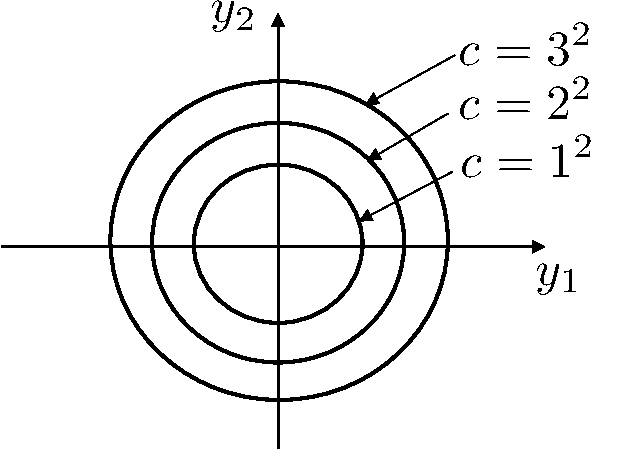
\includegraphics[width=0.5\textwidth]
				{figures/chap6_level_curve_circle}	
		\end{center}
		The level curves of $Q_A(\ybf)$ are circles of radius $\sqrt{c}$.
	\end{example}
\end{frame}


%----------------------------------
\begin{frame}\frametitle{Quadratic Forms}
	\begin{example}
	Consider the quadratic equation
	\[
		f(x) = 2y_1^2 + 3 y_1 y_2 + 4 y_2^2,
	\]	
	and note that
	\begin{align*}
		f(x) 
			&= 2y_1^2 + 3 y_1 y_2 + 4 y_2^2 \\
		 	&= 	\begin{pmatrix}
 					y_1 & y_2 
 				\end{pmatrix}
 				\begin{pmatrix}
 					2y_1 + \frac{3}{2} y_2 \\
 					4y_2 + \frac{3}{2} y_1
 				\end{pmatrix} \\
 		 	&= 	\begin{pmatrix}
 					y_1 & y_2 
 				\end{pmatrix}
 				\begin{pmatrix}
 					2 & \frac{3}{2} \\
 					\frac{3}{2} & 4 
 				\end{pmatrix} 
 				\begin{pmatrix}
 					y_1 \\ y_2	
 				\end{pmatrix} \\
 			&= \ybf^\top A \ybf
	\end{align*}
	\end{example}
	
	Any quadratic equation in $n$ variables can be written in the form $\ybf^\top A \ybf$.
	
\end{frame}


%----------------------------------
\begin{frame}\frametitle{Quadratic Forms}
	By the spectral theorem, $A$ is diagonalizable.  In other words, there exists an invertible $U$ so that 
	$A = U\Lambda U^\top $.
	
	\vfill
	
	From Moon Lemma 6.2 the eigenvalues are real so we can order them as
	\[ 
		\Lambda 
			= \begin{pmatrix}
	    		\lambda_1\\
	    		& \lambda_2\\
	    		& & \ddots\\
	    		& & & \lambda_n
	  		   \end{pmatrix}
	\]
	with
	\[
	  	\lambda_1 \geq \lambda_2 \geq \ldots \geq \lambda_n.
	\]
\end{frame}

%----------------------------------
\begin{frame}\frametitle{Quadratic Forms}
	\begin{lemma}
		Level curves of the quadratic form 
		\[
			Q_A(x-x_0) = (x-x_0)^\top A(x-x_0) = c
		\]
		are hyper-ellipsoids with the length of the axes given by $\frac{1}{\sqrt{\lambda_i}}$.	
	\end{lemma}
	\begin{proofstart}
		Let $z = U^\top y$ then
		\begin{align*}
		 Q_A(y) &= y^\top Ay= y^\top U\Lambda U^\top y = z^\top \Lambda z \\
		 		&= \begin{pmatrix}
		     			z_1 & \cdots & z_n
			   	   \end{pmatrix}
			   	   \begin{pmatrix}
		     			\lambda_1 & & 0\\
		     			& \ddots\\
		     			0 & & \lambda_n
		   			\end{pmatrix}
		   			\begin{pmatrix}
		    			z_1 \\ \vdots \\ z_n
		  			\end{pmatrix} \\
		  		&= \lambda_1 z_1^2 + \dots + \lambda_n z_n^2
		\end{align*}
	\end{proofstart}
\end{frame}

%----------------------------------
\begin{frame}\frametitle{Quadratic Forms}
	\begin{proofcont}
		Note that in the variable $z$, the quadratic form is an ellipsoid:
		\[ 
			Q_A(\ybf)= (\sqrt{\lambda_1})^2z_1^2 + (\sqrt{\lambda_2})^2z_2^2 + \cdots + (\sqrt{\lambda_n})^2z_n^2 = 1 
		\]
		or
		\[ 
			Q_A(\ybf)= \frac{z_1^2}{\left(\frac{1}{\sqrt{\lambda_1}}\right)^2} + \frac{z_2^2}{\left(\frac{1}{\sqrt{\lambda_2}}\right)^2} + \cdots + \frac{z_n^2}{\left(\frac{1}{\sqrt{\lambda_n}}\right)^2} = 1
		\]
		Either of these are the general equation for an ellipsoid with minor axis 
		$\ebf_1 = 	\begin{pmatrix}
						1 & 0 & \cdots & 0 
				  	\end{pmatrix}^\top$ 
		and major axis 
		$\ebf_n = 	\begin{pmatrix} 
						0 & \cdots & 0 & 1
					\end{pmatrix}^\top$
	\end{proofcont}
\end{frame}

%----------------------------------
\begin{frame}\frametitle{Quadratic Forms}
	\begin{columns}
		\begin{column}{0.6\textwidth}
			Note that along $\ebf_1$, the stretching is
			\[ 
				(\sqrt{\lambda_1})^2z_1^2 = 1 \Rightarrow z_1 = \frac{1}{\sqrt{\lambda_1}} 
			\]
			\begin{center}
				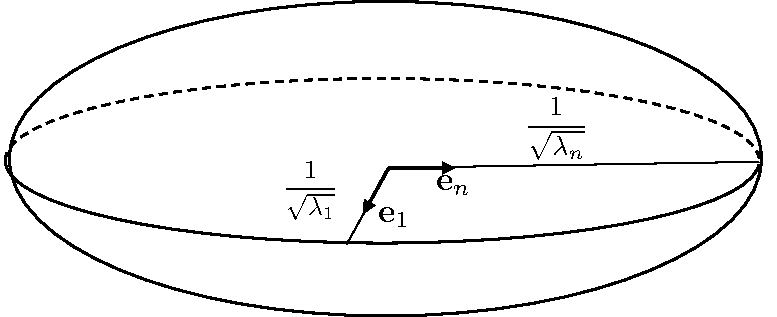
\includegraphics[width=0.99\textwidth]{figures/chap6_quadratic_form_1}
			\end{center}
		\end{column}
		\begin{column}{0.5\textwidth}
			In the original space, what is $\ebf_1$?
			\begin{align*}
				\ebf_1 &= U^\top \ybf 
				    = \begin{pmatrix}
			    		\ubf_1^\top \\
			    		\vdots\\
			    		\ubf_n^\top 
			  		  \end{pmatrix}\ybf \\
			  		&= \begin{pmatrix}
			    		\ubf_1^\top \ybf\\
			    		\vdots\\
			    		\ubf_n^\top \ybf
			  		  \end{pmatrix} 
			  		= \begin{pmatrix}
			    		1\\0\\\vdots\\0
			  		  \end{pmatrix}.
			\end{align*}
			Therefore $\ybf = \ubf_1$ since $U$ is orthogonal.
			
			i.e. $\ubf_i = U \ebf_i$	.
		\end{column}	
	\end{columns}
\end{frame}

%----------------------------------
\begin{frame}\frametitle{Quadratic Forms}
	Therefore the major axis is given by the eigenvector associated with the smallest eigenvalue, and the minor axis is given by the eigenvector associated with the largest eigenvalue.
	
	\vfill
	
	{\color{blue} Question:}  What is the geometric picture associated with
	\[
		(x-x_0)^\top A(x - x_0) = c 
	\]
	where $c$ is a constant and $A$ is symmetric and positive definite?
	
	\vfill
	
	{\color{blue} Answer:}  An ellipsoid of radius $\sqrt{c}$ centered at $x_0$ with axes along the eigenvectors of $A$ and stretching along each axis given by $\displaystyle \frac{1}{\sqrt{\lambda_i}}$.
\end{frame}

%----------------------------------
\begin{frame}\frametitle{Quadratic Forms}
	{\color{blue}Question:}  
	What if we would like to maximize
	\[ 
		Q_A(y) = y^\top Ay \text{ where } \norm{y} = 1.
	\]
	Which axis provides the most bang-for-the-buck?
	
	\vfill
	
	{\color{blue}Answer:} The \underline{major} axis!  i.e. the axis associated with the largest eigenvalue.
	
\end{frame}

%----------------------------------
\begin{frame}\frametitle{Quadratic Forms}
	Rather than drawing
	\[ 
		\lambda_1 z_1^2 + \lambda_2 z_2^2 + \cdots + \lambda_n z_n^2 = 1 
	\]
	which is
	\begin{center}
		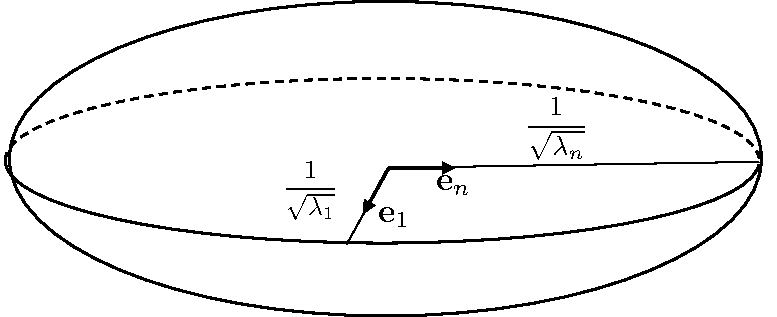
\includegraphics[width=0.5\textwidth]{figures/chap6_quadratic_form_1}
	\end{center}
	lets draw the mapping of the unit circle through $\ybf^\top A\ybf$
	i.e.
	\[ 
		\{ \norm{\ybf}=1 \} 
			\overset{Q_A(\ybf)}{\longrightarrow} 
		\{ \ybf^\top A \ybf \}
	\]
	\begin{center}
		
\includegraphics[width=0.5\textwidth]
			{figures/chap6_mapping_1}
	\end{center}
\end{frame}

%----------------------------------
\begin{frame}\frametitle{Quadratic Forms}
	If $A=A^\top $ then $A=U\Lambda U^\top $ where $U$ is orthogonal, i.e., $UU^\top =U^\top U=I$.
	Then
	\begin{align*}
		\max_{\norm{\ybf}=1} \ybf^\top  A \ybf 
			&= \max_{\norm{\ybf}=1} \ybf^\top  U \Lambda U^\top  \ybf.	
	\end{align*}
	
	\vfill

	Let $\zbf=U^\top  \ybf$ and note that $\norm{\zbf}=\norm{U^\top  \ybf} = \norm{\ybf}$ since $U$ is orthogonal.
	Then 
	\begin{align*}
		\max_{\norm{\ybf}=1} \ybf^\top  U \Lambda U^\top  \ybf 
			&= \max_{\norm{\zbf}=1} \zbf^\top  \Lambda \zbf \\
			&= \max_{\norm{\zbf}=1} \left( \lambda_1 z_1^1 + \lambda_2 z_2^2 + \cdots + \lambda_n z_n^2 \right)	
	\end{align*}
	where $\Lambda$ is arranged such that
	\[
	\lambda_1 \geq \lambda_2 \geq \cdots \geq \lambda_n.
	\]
\end{frame}

%----------------------------------
\begin{frame}\frametitle{Quadratic Forms}
	The maximum is therefore 
	\[
	\zbf^\ast = \begin{pmatrix} 1 & 0 & \vdots & 0 \end{pmatrix}^\top
	\]
	where it is clear that $\norm{\zbf}=1$.
	
	Furthermore
	\[
		\max_{\norm{\zbf}=1} \zbf^\top  \Lambda \zbf = \lambda_1,
	\]
	which implies that
	\[
	\ybf^\ast = U\zbf^\ast = \begin{pmatrix} \ubf_1 & \cdots & \ubf_n \end{pmatrix} \begin{pmatrix} 1 \\ 0 \\ \vdots \\ 0 \end{pmatrix} = \ubf_1.
	\]	
\end{frame}

%----------------------------------
\begin{frame}\frametitle{Quadratic Forms}
	This mapping also forms an ellipsoid but with a different effect.
	
	Let $\ybf = \ubf_1 \implies \norm{\ybf} = 1 $ to get
	\[ 
		Q_A(\ybf) = \lambda_1 
	\]
	
	\vfill
	
	{\color{blue}Question:} 
	Is it possible to pick a $\hat{\ybf}$ where $\norm{\hat{\ybf}} = 1$ such that 
	\[
		Q_A(\hat{\ybf}) > Q_A(\ubf_1)?
	\]
	
	\vfill
	
	{\color{blue}Answer:} No.
	
\end{frame}

%----------------------------------
\begin{frame}\frametitle{Quadratic Forms}
	{\color{blue}Explanation:}
	Recall that $\lambda_1 \geq \lambda_2 \geq \ldots \geq \lambda_n$ and $\norm{\hat{\ybf} } = y_1^2 + \cdots + y_n^2 = 1$.
	
	\vfill
	
	Therefore
	\begin{align*}
		Q_A(\hat{\ybf}) 
			&= \lambda_1y_1^2 + \cdots + \lambda_ny_n^2 \\
			&\leq \lambda_1y_1^2 + \lambda_1y_2^2 + \cdots + \lambda_1y_n^2 \\
		&= \lambda_1\norm{\hat{\ybf}}^2 \\
		&= Q_A(\ubf_1)
	\end{align*}
	So the mapping of the unit circle looks like
	\begin{center}
		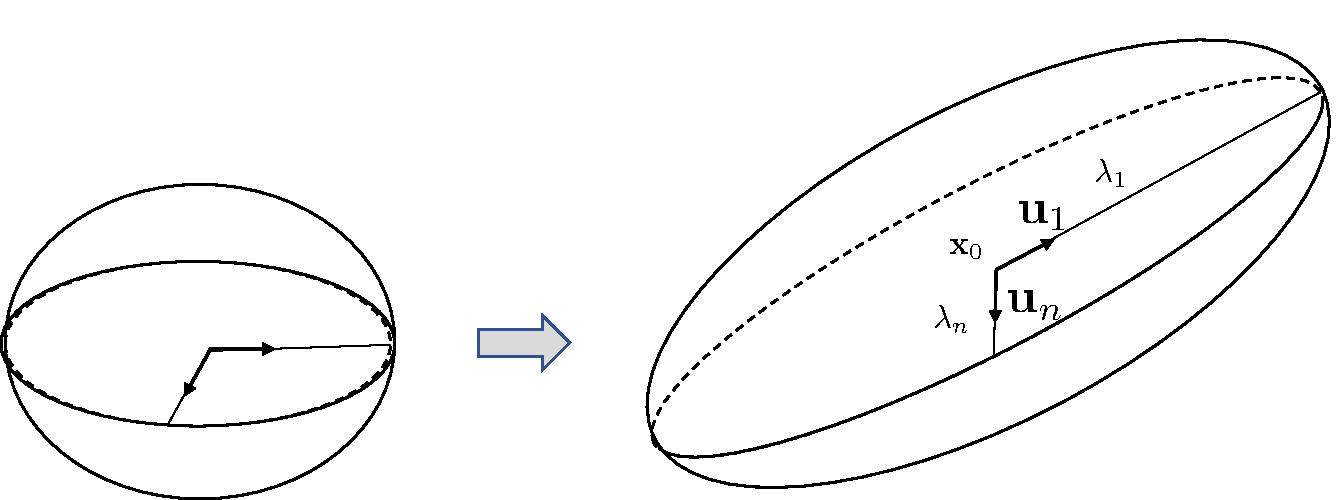
\includegraphics[width=0.6\textwidth]
			{figures/chap6_mapping_2}
	\end{center}
\end{frame}

%----------------------------------
\begin{frame}\frametitle{Quadratic Forms}
	We have essentially proved the following theorem:
	\begin{theorem}[Moon Theorem 6.5]
		For a positive semi-definite Hermitian matrix $A$, the maximum
		\[ 
			\lambda_1 = \max_{\norm{\xbf}_2=1} \xbf^H A \xbf 
		\]
		where $\lambda_1$ is the largest eigenvalue of $A$, and the maximizing $\xbf$ is $\xbf = \ubf_1$, the associated eigenvector.
		
		\vfill
		
		Furthermore if we maximize $\xbf^H A \xbf$ subject to the constraints
		\begin{align*}
			\iprod{\xbf, \ubf_i} &= 0 \qquad i = 1,\ldots,k-1, \\
			\norm{\xbf}_2 &= 1 
		\end{align*}
		then the maximum is $\lambda_k$ and $\xbf_{max} = \ubf_k$.		
	\end{theorem}
\end{frame}

%----------------------------------
\begin{frame}\frametitle{Quadratic Forms}
	Note that if $A$ is positive semi-definite Hermitian then
	\begin{align*}
		\norm{A}_2 
			= \sup_{\norm{\xbf}_2\neq 0}\frac{\norm{A\xbf}_2}{\norm{\xbf}_2} 
			= \max_{\norm{\xbf}_2 = 1} \sqrt{\xbf^H A^H A\xbf} 
			= \sqrt{\lambda_1 \ubf_1^H \ubf_1} 
			= \sqrt{\lambda_1} 
	\end{align*}
	where $\lambda_1$ is the largest eigenvalue of $A^H A$.
	
	\vfill
	
	More generally,
	\[ 
		R(x) = \frac{\xbf^\top A\xbf}{\xbf^\top \xbf} 
	\] 
	is called a Rayleigh quotient and
	\begin{align*}
		\max_{\norm{\xbf}\neq 0} R(\xbf) &= \lambda_1 \\
		\min_{\norm{\xbf}\neq 0} R(\xbf) &= \lambda_n.
	\end{align*}
\end{frame}



%%%%%%%%%%%%%%%%%%%%%%%%%%%%%%%%%%%%%%%%%%%%%%%%%%%%%%%%%%%%%%%%%
\section{Eigenfilters}
\frame{\sectionpage}

%----------------------------------
\begin{frame}\frametitle{Eigenfilters for Random Signals}
	{\color{blue}Problem:}
	Given
	\begin{center}
		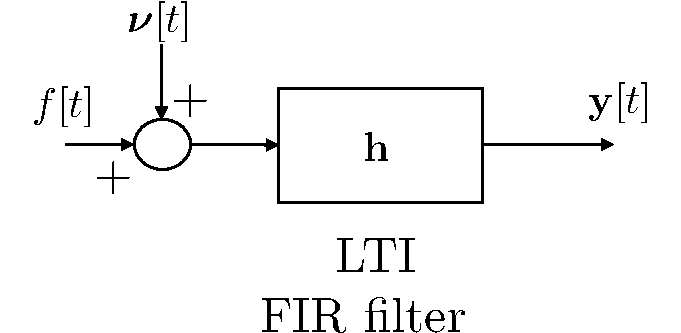
\includegraphics[width=0.6\textwidth]{figures/chap6_eigenfilter}
	\end{center}
	where $\nu$ is white noise with variance $\sigma^2$, and $f$ is a stationary, zero-mean random process.
	
	\vfill
	
	Find $\mathbf{h}$ to maximize the signal-to-noise ratio.
\end{frame}

%----------------------------------
\begin{frame}\frametitle{Eigenfilters for Random Signals}
	Let
	\[
		\fbf(t) 
			= \begin{pmatrix}
	    		f(t)\\
	    		f(t-1)\\
	    		\vdots\\
	    		f(t-(m-1))
	  		  \end{pmatrix}
	\]
	then
	\[ 
		y(t) = \hbf^H \fbf(t).
	\]
	The output power due to the signal $\fbf$ is 
	\begin{align*}
		P_0 
		&= E|y(t)|^2 = E|\hbf^H\fbf(t)|^2 = E\{\hbf^H\fbf(t)\hbf^H\fbf(t)\}\\
		&= E\{\hbf^H\fbf(t)\fbf^H(t)\hbf\}= \hbf^HE\{\fbf(t)\fbf^H(t)\}\hbf\\
		&= \hbf^HR\hbf
	\end{align*}
	
	where $R = E\{\fbf(t) \fbf^H(t)\} $
\end{frame}

%----------------------------------
\begin{frame}\frametitle{Eigenfilters for Random Signals}
	Let 
	\[ 
		\nubf(t) 
			= \begin{pmatrix}
	    		v(t)\\
	    		v(t-1)\\
	    		\vdots
	    		\\
	    		v(t-m+1)
	  		  \end{pmatrix}
	\]
	Then the output due to the noise is
	\[ 
		\hbf\nubf(t) 
	\]
	and the average noise power is
	\[ 
		N_0 = E\{\hbf^H\nubf(t)\nubf^H(t)\hbf\} 
		    = \sigma^2\hbf^H\hbf 
	\]
\end{frame}

%----------------------------------
\begin{frame}\frametitle{Eigenfilters for Random Signals}
	The signal-to-noise ratio is
	\begin{align*}
		SNR &= \frac{P_0}{N_0} \\
		    &= \frac{1}{\sigma^2} \cdot
		    	\underbrace{
		    		\frac{\hbf^HR\hbf}{\sigma^2\hbf^H\hbf}
		    	}_{\text{Rayleigh quotient}} 
	\end{align*}
	Therefore
	\[ 
		SNR_{max} = \frac{\lambda_1}{\sigma^2} 
	\]
	where $\lambda_1$ is the largest eigenvalue of $R$ and $\hbf = q_1$ the largest eigenvector of $R$.
\end{frame}

\end{document}
